% Author: Izaak Neutelings (March 2020)
\documentclass[border=3pt,tikz]{standalone}
\usepackage{amsmath} % for \dfrac
\usepackage{mathabx} % for \Earth
\usepackage{bm} % \bm
\usepackage{physics}
\usepackage{tikz}
\usetikzlibrary{arrows.meta}
\usetikzlibrary{calc}
\tikzset{>=latex} % for LaTeX arrow head
\usepackage{xcolor}
\colorlet{vcol}{red!50!black}
\colorlet{veccol}{green!50!black}
\colorlet{Icol}{blue!70!black}
\colorlet{wcol}{orange!90!black}
\colorlet{Scol}{green!60!black}
\tikzstyle{current}=[->,Icol] %thick,
\tikzstyle{force}=[->,very thick,BFcol]
\tikzstyle{velocity}=[->,thick,vcol]
\tikzstyle{spin}=[->,very thick,Scol]
\tikzstyle{charge+}=[very thin,draw=black,top color=red!50,bottom color=red!90!black,shading angle=20,circle,inner sep=0.2]
\tikzstyle{charge-}=[very thin,draw=black,top color=blue!50,bottom color=blue!80,shading angle=20,circle,inner sep=0.2]
\tikzstyle{charge0}=[very thin,draw=black,top color=green!60!black!40,bottom color=green!60!black!80,shading angle=20,circle,inner sep=0.2]
\tikzstyle{vector}=[->,thick,veccol]
\tikzset{
  pics/spin/.style={
    code={
      \def\L{0.38}
      \draw[-{Latex[length=3,width=2.5]},pic actions,rotate=#1,line width=0.9,Scol] (-\L/2,0) --++ (\L,0);
      \draw[pic actions,rotate=#1,thin,white]
        (-0.15*\L,0)++(170:{0.16*\L} and {0.22*\L}) arc (170:190:{0.16*\L} and {0.22*\L});
      \draw[-{Latex[length=1.2,width=1]},pic actions,rotate=#1,very thin]
        (-0.15*\L,0)++(25:{0.16*\L} and {0.22*\L}) arc (25:305:{0.16*\L} and {0.22*\L}) --++ (50:0.09*\L);
  }},
  pics/spin/.default=90,
}



\begin{document}



% PION DECAY
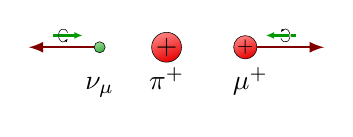
\begin{tikzpicture}
  \def\L{1.0}
  \def\v{0.9*\L}
  \coordinate (O) at (0,0);
  \coordinate (L) at (-0.85*\L,0);
  \coordinate (R) at (\L,0);
  \coordinate (LS) at ($(L)+(-0.45*\v,0.15*\L)$);
  \coordinate (RS) at ($(R)+( 0.50*\v,0.15*\L)$);
  
  % VECTORS
  \draw[->,velocity] (R)++(0.1*\L,0) --++ (\v,0);
  \draw[->,velocity] (L) --++ (-\v,0);
  \pic at (RS) {spin={180}};
  \pic at (LS) {spin={  0}};
  %\node[vcol,above=5,scale=0.8] at (O) {$S_\pi = 0$};
  
  % PARTICLES
  \draw[charge0] (L) circle (0.07*\L);
  \node[charge+,scale=1.00] at (O) {$+$};
  \node[charge+,scale=0.78] at (R) {$+$};
  \node at ($(L)+(0,-0.45*\L)$) {\strut$\nu_\mu$};
  \node at ($(O)+(0,-0.45*\L)$) {\strut$\pi^+$};
  \node[right=-8] at ($(R)+(0,-0.45*\L)$) {\strut$\mu^+$};
  
\end{tikzpicture}



% MU DECAY - maximal positron energy
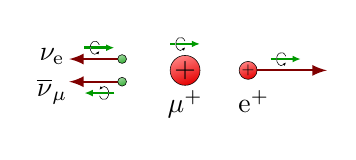
\begin{tikzpicture}
  \def\L{0.8}
  \def\v{1.2*\L}
  \coordinate (O) at (0,0);
  \coordinate (LT) at (-\L, 0.18*\L);
  \coordinate (LB) at (-\L,-0.18*\L);
  \coordinate (R) at (\L,0);
  \coordinate (T) at (0,0.42*\L);
  \coordinate (LTS) at ($(LT)+(-0.3*\v, 0.18*\L)$);
  \coordinate (LBS) at ($(LB)+(-0.3*\v,-0.18*\L)$);
  \coordinate (RS) at ($(R)+( 0.50*\v,0.18*\L)$);
  
  % VECTORS
  \draw[->,velocity] (R)++(0.05*\L,0) --++ (\v,0);
  \draw[->,velocity] (LT) --++ (-0.7*\v,0) node[black,above=2,left=-2] {\strut$\nu_\mathrm{e}$};
  \draw[->,velocity] (LB) --++ (-0.7*\v,0) node[black,below=3,left=-3] {\strut$\overline{\nu}_\mu$};
  \pic at (RS)  {spin={  0}};
  \pic at (LTS) {spin={  0}};
  \pic at (LBS) {spin={180}};
  \pic at (T)   {spin={  0}};
  
  % PARTICLES
  \draw[charge0] (LT) circle (0.07*\L);
  \draw[charge0] (LB) circle (0.07*\L);
  \node[charge+,scale=1.00] at (O) {$+$};
  \node[charge+,scale=0.60] at (R) {$+$};
  \node at ($(O)+(0,-0.56*\L)$) {\strut$\mu^+$};
  \node[right=-7] at ($(R)+(0,-0.56*\L)$) {\strut$\mathrm{e}^+$};
  
\end{tikzpicture}



% MU DECAY - minimal positron energy
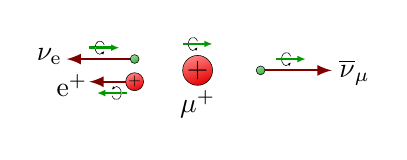
\begin{tikzpicture}
  \def\L{0.8}
  \def\v{1.2*\L}
  \coordinate (O) at (0,0);
  \coordinate (LT) at (-\L, 0.18*\L);
  \coordinate (LB) at (-\L,-0.18*\L);
  \coordinate (R) at (\L,0);
  \coordinate (T) at (0,0.42*\L);
  \coordinate (LTS) at ($(LT)+(-0.4*\v, 0.18*\L)$);
  \coordinate (LBS) at ($(LB)+(-0.3*\v,-0.18*\L)$);
  \coordinate (RS) at ($(R)+( 0.4*\v,0.18*\L)$);
  
  % VECTORS
  \draw[->,velocity] (R)++(0.05*\L,0) --++ (0.9*\v,0) node[black,right=-1] {\strut$\overline{\nu}_\mu$};
  \draw[->,velocity] (LT) --++ (-0.9*\v,0) node[black,above=2,left=-2] {\strut$\nu_\mathrm{e}$};
  \draw[->,velocity] (LB) --++ (-0.6*\v,0) node[black,below=3,left=-3] {\strut$\mathrm{e}^+$};
  \pic at (RS)  {spin={  0}};
  \pic at (LTS) {spin={  0}};
  \pic at (LBS) {spin={180}};
  \pic at (T)   {spin={  0}};
  
  % PARTICLES
  \draw[charge0] (LT) circle (0.07*\L);
  \draw[charge0] (R) circle (0.07*\L);
  \node[charge+,scale=1.00] at (O) {$+$};
  \node[charge+,scale=0.60] at (LB) {$+$};
  \node at ($(O)+(0,-0.56*\L)$) {\strut$\mu^+$};
  
\end{tikzpicture}



\end{document}
